% !TEX encoding = UTF-8 Unicode
% !TEX root = ../rapport.tex

\chapter{Algorithme d'exclusion mutuelle de Naimi-Trehel}\label{naimi-trehel}


\section{Description}
L'algorithme de Naimi-Trehel \cite{naimi1996} est basé sur le fait de conserver deux structures de données distribuées et un jeton. Le jeton est présent sur un des sites à la fois et matérialise la permission d'entrer en section critique. Les structures de données distribuées sont un arbre logique dynamique et une file d'attente.

La file d'attente stocke les sites qui ont demandé à entrer en section critique. La file d'attente étant distribuée, chaque site stocke uniquement son suivant (s'il y en a un) dans la file d'attente. La tête de la file est le site actuellement en section critique et la queue de la file est le dernier site à avoir demandé à y entrer. Quand un site demande à entrer en section critique, il est ajouté à la fin de la file. Quand un site quitte la section critique, il envoie le jeton à son suivant dans la file (s'il y en a un).

La seconde structure de données est l'arbre logique dynamique. Cet arbre a pour but d'indiquer aux sites lequel d'entre eux est le dernier dans la file d'attente. La structure étant distribuée, chaque site stocke uniquement son père dans l'arbre. Lorsqu'un site veut entrer en section critique, il transmet la requête à son père qui (s'il n'est pas racine) transmet la requête à son père jusqu'à ce que la requête atteigne la racine de l'arbre. Le site racine dans l'arbre étant également le dernier dans la file d'attente, il fixe son suivant au site qui a émis la requête. Puis tous les sites qui ont transmis la requête fixent leur père au site qui a émis la requête (désormais le dernier dans la file d'attente).


\section{Exemple}

\tikzstyle{vertex}=[circle,fill=black!25,minimum size=20pt,inner sep=0pt]
\tikzstyle{edge} = [draw,thick,-]
\tikzstyle{tree edge} = [draw, thick,->,red!75]
\tikzstyle{queue edge} = [draw,thick,->,blue!50]

Dans cet exemple, initialement, le nœud $a$ possède le jeton (figure \ref{naimi-trehel-exemple1}).
\begin{figure}[H]
	\centering
	\subfigure[Réseau physique]
	{
		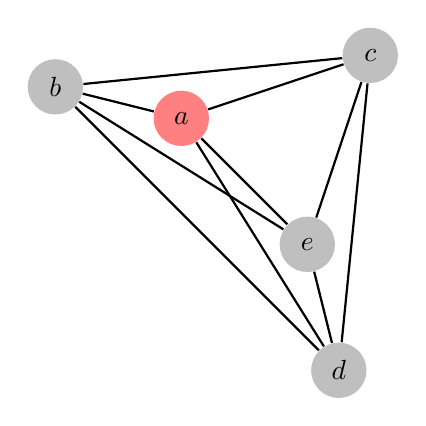
\begin{tikzpicture}[scale=0.8,auto,swap]
			\node[vertex,fill=red!50] (a) at (2,4) {$a$};
			\node[vertex] (b) at (0,4.5) {$b$};
			\node[vertex] (c) at (5,5) {$c$};
			\node[vertex] (d) at (4.5,0) {$d$};
			\node[vertex] (e) at (4,2) {$e$};
    			% First we draw the vertices
			\draw (a) (b) (c) (d) (e);
   			 % Connect vertices with edges
   			\foreach \source/ \dest in {a/b, a/c, a/d, a/e, b/c, b/d, b/e, c/d, c/e, d/e}
        			\path[edge] (\source) -- (\dest);
		\end{tikzpicture}
	}
	\subfigure[Arbre logique]
	{
		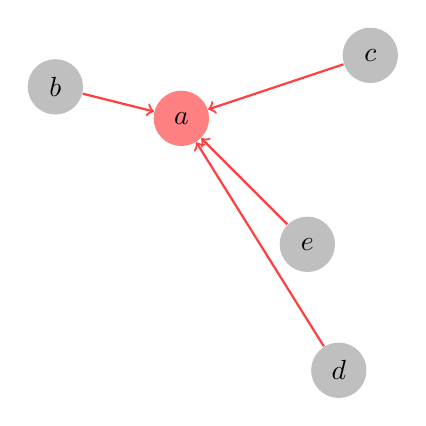
\begin{tikzpicture}[scale=0.8,auto,swap]
		\node[vertex,fill=red!50] (a) at (2,4) {$a$};
		\node[vertex] (b) at (0,4.5) {$b$};
		\node[vertex] (c) at (5,5) {$c$};
		\node[vertex] (d) at (4.5,0) {$d$};
		\node[vertex] (e) at (4,2) {$e$};
    		% First we draw the vertices
		\draw (a) (b) (c) (d) (e);
   		 % Connect vertices with edges
   		 \foreach \source/ \dest in {b/a, c/a, d/a, e/a}
		 \path[tree edge] (\source) to (\dest);
		\end{tikzpicture}
	}
	\subfigure[File d'attente]
	{
		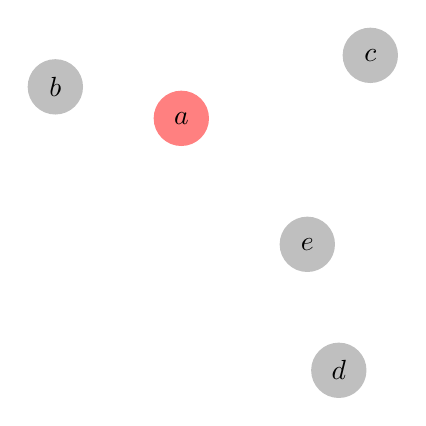
\begin{tikzpicture}[scale=0.8,auto,swap]
		\node[vertex,fill=red!50] (a) at (2,4) {$a$};
		\node[vertex] (b) at (0,4.5) {$b$};
		\node[vertex] (c) at (5,5) {$c$};
		\node[vertex] (d) at (4.5,0) {$d$};
		\node[vertex] (e) at (4,2) {$e$};
    		% First we draw the vertices
		\draw (a) (b) (c) (d) (e);
		\end{tikzpicture}
	}
	\caption{\label{naimi-trehel-exemple1}}
\end{figure}

Puis le nœud $b$ fait une requête pour obtenir la section critique. Il envoie cette requête au nœud $a$ et deviens la nouvelle racine. Le site $a$ reçoit la requête venant de $b$ et lui envoie le jeton. Le père de $a$ dans l'arbre devient $b$. Le site $b$ reçoit le jeton et entre en section critique. (figure \ref{naimi-trehel-exemple2})

\begin{figure}[H]
\centering
	\subfigure[Réseau physique]
	{
		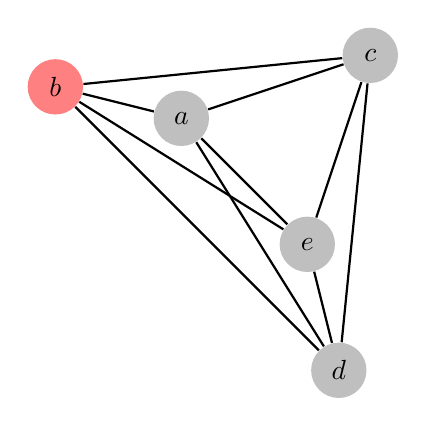
\begin{tikzpicture}[scale=0.8,auto,swap]
			\node[vertex] (a) at (2,4) {$a$};
			\node[vertex,fill=red!50] (b) at (0,4.5) {$b$};
			\node[vertex] (c) at (5,5) {$c$};
			\node[vertex] (d) at (4.5,0) {$d$};
			\node[vertex] (e) at (4,2) {$e$};
	    		% First we draw the vertices
			\draw (a) (b) (c) (d) (e);
	   		 % Connect vertices with edges
	   		\foreach \source/ \dest in {a/b, a/c, a/d, a/e, b/c, b/d, b/e, c/d, c/e, d/e}
	        		\path[edge] (\source) -- (\dest);
		\end{tikzpicture}
	}
	\subfigure[Arbre logique]
	{
		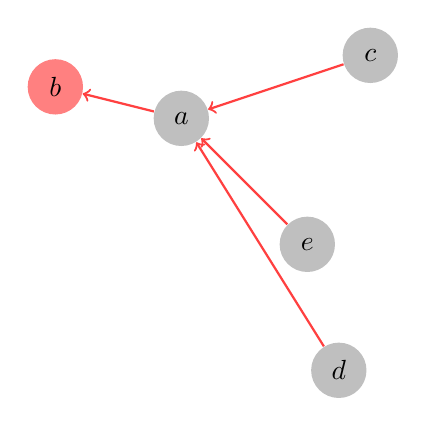
\begin{tikzpicture}[scale=0.8,auto,swap]
			\node[vertex] (a) at (2,4) {$a$};
			\node[vertex,fill=red!50] (b) at (0,4.5) {$b$};
			\node[vertex] (c) at (5,5) {$c$};
			\node[vertex] (d) at (4.5,0) {$d$};
			\node[vertex] (e) at (4,2) {$e$};
	    		% First we draw the vertices
			\draw (a) (b) (c) (d) (e);
	   		 % Connect vertices with edges
	   		 \foreach \source/ \dest in {a/b, c/a, d/a, e/a}
			 \path[tree edge] (\source) to (\dest);
		\end{tikzpicture}
	}
	\subfigure[File d'attente]
	{
		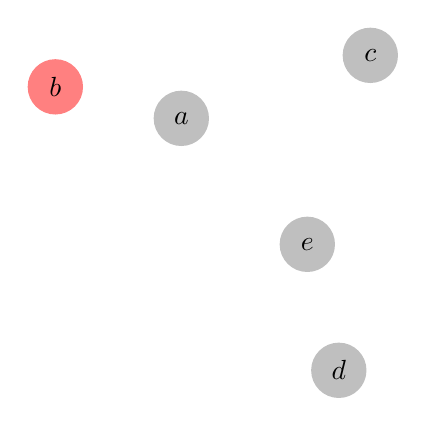
\begin{tikzpicture}[scale=0.8,auto,swap]
			\node[vertex] (a) at (2,4) {$a$};
			\node[vertex,fill=red!50] (b) at (0,4.5) {$b$};
			\node[vertex] (c) at (5,5) {$c$};
			\node[vertex] (d) at (4.5,0) {$d$};
			\node[vertex] (e) at (4,2) {$e$};
	    		% First we draw the vertices
			\draw (a) (b) (c) (d) (e);
		\end{tikzpicture}
	}
	\caption{\label{naimi-trehel-exemple2}}
\end{figure}

Le site $c$ demande à entrer en section critique. Il envoie une requête au nœud $a$ qui la transmet au nœud $b$. Le nœud $b$ reçoit la requête et considère $c$ comme son suivant dans la file d'attente. $a$ et $b$ fixent $c$ comme leur père dans l'arbre. (figure \ref{naimi-trehel-exemple3})

\begin{figure}[H]
\centering
	\subfigure[Réseau physique]
	{
		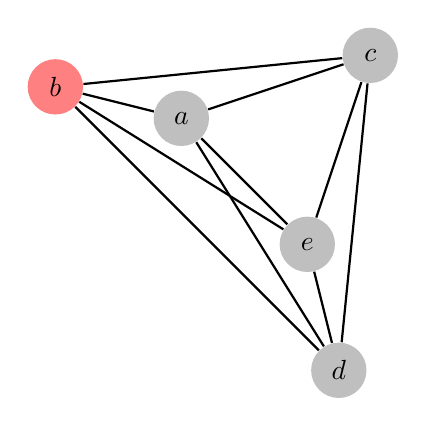
\begin{tikzpicture}[scale=0.8,auto,swap]
			\node[vertex] (a) at (2,4) {$a$};
			\node[vertex,fill=red!50] (b) at (0,4.5) {$b$};
			\node[vertex] (c) at (5,5) {$c$};
			\node[vertex] (d) at (4.5,0) {$d$};
			\node[vertex] (e) at (4,2) {$e$};
	    		% First we draw the vertices
			\draw (a) (b) (c) (d) (e);
	   		 % Connect vertices with edges
	   		\foreach \source/ \dest in {a/b, a/c, a/d, a/e, b/c, b/d, b/e, c/d, c/e, d/e}
	        		\path[edge] (\source) -- (\dest);
		\end{tikzpicture}
	}
	\subfigure[Arbre logique]
	{
		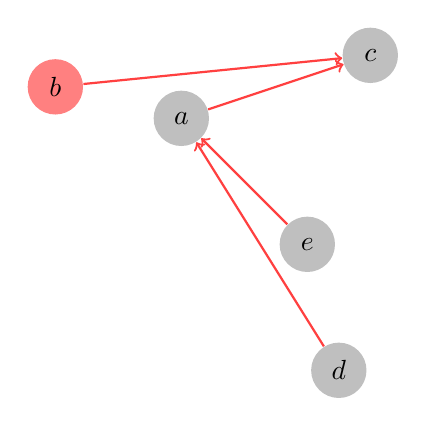
\begin{tikzpicture}[scale=0.8,auto,swap]
			\node[vertex] (a) at (2,4) {$a$};
			\node[vertex,fill=red!50] (b) at (0,4.5) {$b$};
			\node[vertex] (c) at (5,5) {$c$};
			\node[vertex] (d) at (4.5,0) {$d$};
			\node[vertex] (e) at (4,2) {$e$};
	    		% First we draw the vertices
			\draw (a) (b) (c) (d) (e);
	   		 % Connect vertices with edges
	   		 \foreach \source/ \dest in {a/c, b/c, d/a, e/a}
			 \path[tree edge] (\source) to (\dest);
		\end{tikzpicture}
	}
	\subfigure[File d'attente]
	{
		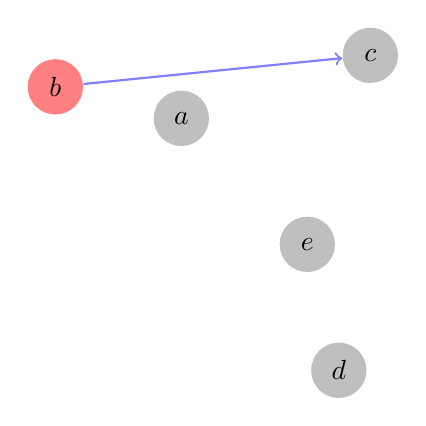
\begin{tikzpicture}[scale=0.8,auto,swap]
			\node[vertex] (a) at (2,4) {$a$};
			\node[vertex,fill=red!50] (b) at (0,4.5) {$b$};
			\node[vertex] (c) at (5,5) {$c$};
			\node[vertex] (d) at (4.5,0) {$d$};
			\node[vertex] (e) at (4,2) {$e$};
	    		% First we draw the vertices
			\draw (a) (b) (c) (d) (e);
	   		 % Connect vertices with edges
	   		\foreach \source/ \dest in {b/c}
	        		\path[queue edge] (\source) to (\dest);
		\end{tikzpicture}
	}
	\caption{\label{naimi-trehel-exemple3}}
\end{figure}

Le site $d$ demande à entrer en section critique. Il envoie une requête au site $a$ qui transmet au site $c$. Le site $c$ reçoit la requête relayée par le site $a$, son suivant dans la file devient $d$, son père également. Le père de $a$ devient $d$. (figure \ref{naimi-trehel-exemple4})

\begin{figure}[H]
\centering
	\subfigure[Réseau physique]
	{
		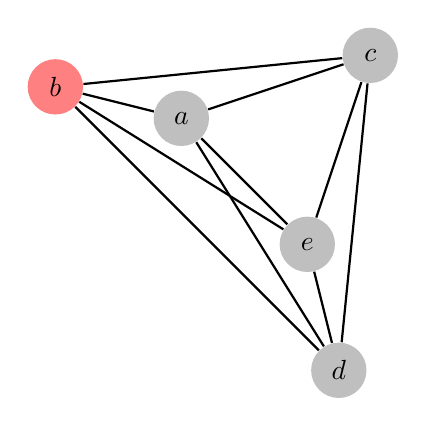
\begin{tikzpicture}[scale=0.8,auto,swap]
			\node[vertex] (a) at (2,4) {$a$};
			\node[vertex,fill=red!50] (b) at (0,4.5) {$b$};
			\node[vertex] (c) at (5,5) {$c$};
			\node[vertex] (d) at (4.5,0) {$d$};
			\node[vertex] (e) at (4,2) {$e$};
	    		% First we draw the vertices
			\draw (a) (b) (c) (d) (e);
	   		 % Connect vertices with edges
	   		\foreach \source/ \dest in {a/b, a/c, a/d, a/e, b/c, b/d, b/e, c/d, c/e, d/e}
	        		\path[edge] (\source) -- (\dest);
		\end{tikzpicture}
	}
	\subfigure[Arbre logique]
	{
		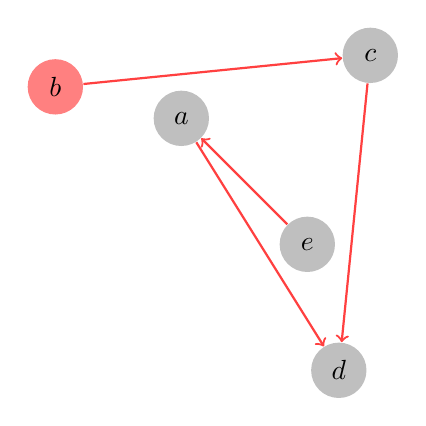
\begin{tikzpicture}[scale=0.8,auto,swap]
			\node[vertex] (a) at (2,4) {$a$};
			\node[vertex,fill=red!50] (b) at (0,4.5) {$b$};
			\node[vertex] (c) at (5,5) {$c$};
			\node[vertex] (d) at (4.5,0) {$d$};
			\node[vertex] (e) at (4,2) {$e$};
	    		% First we draw the vertices
			\draw (a) (b) (c) (d) (e);
	   		 % Connect vertices with edges
	   		 \foreach \source/ \dest in {a/d, c/d, b/c, e/a}
			 \path[tree edge] (\source) to (\dest);
		\end{tikzpicture}
	}
	\subfigure[File d'attente]
	{
		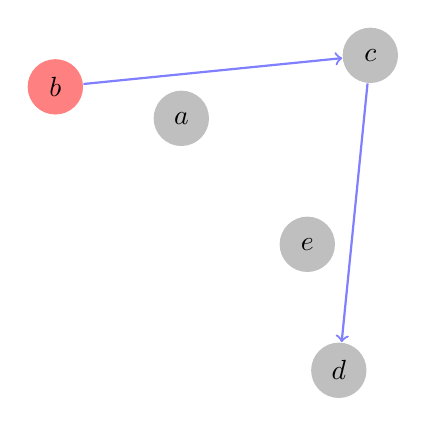
\begin{tikzpicture}[scale=0.8,auto,swap]
			\node[vertex] (a) at (2,4) {$a$};
			\node[vertex,fill=red!50] (b) at (0,4.5) {$b$};
			\node[vertex] (c) at (5,5) {$c$};
			\node[vertex] (d) at (4.5,0) {$d$};
			\node[vertex] (e) at (4,2) {$e$};
	    		% First we draw the vertices
			\draw (a) (b) (c) (d) (e);
	   		 % Connect vertices with edges
	   		\foreach \source/ \dest in {b/c, c/d}
	        		\path[queue edge] (\source) to (\dest);
		\end{tikzpicture}
	}
	\caption{\label{naimi-trehel-exemple4}}
\end{figure}

Le site $b$ relâche la section critique et envoie le jeton à son suivant : $c$.
\begin{figure}[H]
\centering
	\subfigure[Réseau physique]
	{
		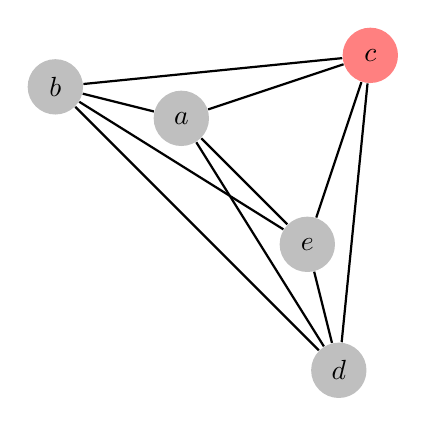
\begin{tikzpicture}[scale=0.8,auto,swap]
			\node[vertex] (a) at (2,4) {$a$};
			\node[vertex] (b) at (0,4.5) {$b$};
			\node[vertex,fill=red!50] (c) at (5,5) {$c$};
			\node[vertex] (d) at (4.5,0) {$d$};
			\node[vertex] (e) at (4,2) {$e$};
	    		% First we draw the vertices
			\draw (a) (b) (c) (d) (e);
	   		 % Connect vertices with edges
	   		\foreach \source/ \dest in {a/b, a/c, a/d, a/e, b/c, b/d, b/e, c/d, c/e, d/e}
	        		\path[edge] (\source) -- (\dest);
		\end{tikzpicture}
	}
	\subfigure[Arbre logique]
	{
		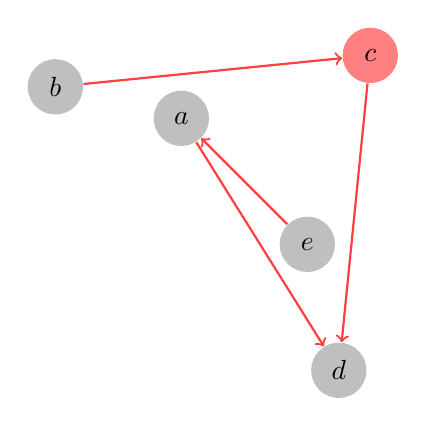
\begin{tikzpicture}[scale=0.8,auto,swap]
			\node[vertex] (a) at (2,4) {$a$};
			\node[vertex] (b) at (0,4.5) {$b$};
			\node[vertex,fill=red!50] (c) at (5,5) {$c$};
			\node[vertex] (d) at (4.5,0) {$d$};
			\node[vertex] (e) at (4,2) {$e$};
	    		% First we draw the vertices
			\draw (a) (b) (c) (d) (e);
	   		 % Connect vertices with edges
	   		 \foreach \source/ \dest in {a/d, c/d, b/c, e/a}
			 \path[tree edge] (\source) to (\dest);
		\end{tikzpicture}
	}
	\subfigure[File d'attente]
	{
		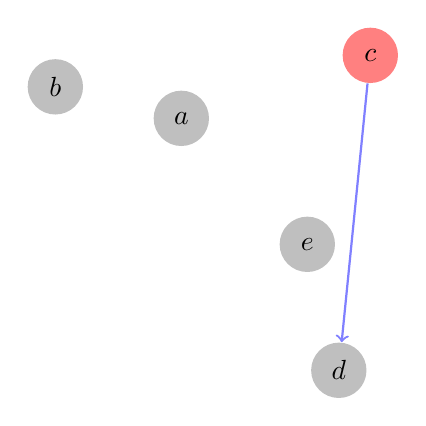
\begin{tikzpicture}[scale=0.8,auto,swap]
			\node[vertex] (a) at (2,4) {$a$};
			\node[vertex] (b) at (0,4.5) {$b$};
			\node[vertex,fill=red!50] (c) at (5,5) {$c$};
			\node[vertex] (d) at (4.5,0) {$d$};
			\node[vertex] (e) at (4,2) {$e$};
	    		% First we draw the vertices
			\draw (a) (b) (c) (d) (e);
	   		 % Connect vertices with edges
	   		\foreach \source/ \dest in {c/d}
	        		\path[queue edge] (\source) to (\dest);
		\end{tikzpicture}
	}
	\caption{\label{naimi-trehel-exemple4}}
\end{figure}


\section{Propriétés}
La première des propriétés que respecte cet algorithme est la sureté. En effet, il est nécessaire qu'au plus un processus à la fois entre en section critique. Ceci est garanti par la présence du jeton. Ce jeton est initialement présent chez un seul site. Lors du déroulement de l'algorithme, il y a deux possibilités pour qu'un autre site reçoive le jeton : 
\begin{itemize}
	\item soit le site qui possède le jeton sort de la section critique avec un suivant non-nul. Il lui envoie alors le jeton et le perd pour lui-même.
	\item soit le site qui possède le jeton reçoit une demande et n'est pas lui-même en section critique. Il envoie alors le jeton et le perd pour lui-même.
\end{itemize}
Dans les deux cas, l'unicité du jeton est préservée et l'exclusion mutuelle est garantie.

La seconde propriété est la vivacité c'est à dire le fait que tout site demandant à entrer en section critique le puisse dans un temps fini. Cette propriété est respectée grâce à l'arbre logique et à la file d'attente. En effet, chaque site voulant entrer en section critique fait la requête à son père dans l'arbre. Le fait que la structure d'arbre distribué soit toujours valide garantie que les requêtes parviennent à la racine de l'arbre. Or la racine de l'arbre étant le dernier nœud de la file d'attente, le site ayant fait la requête se retrouve le dernier dans la file d'attente. Par conséquent, quand son prédécesseur dans la file sortira de la section critique, il pourra y entrer. Dans l'hypothèse où un site ne reste pas éternellement en section critique, la propriété de vivacité est respectée par l'algorithme de Naimi-Trehel.

Cependant cet algorithme n'étant pas parfait, il ne respecte pas l'ordre des demandes et n'est pas nativement tolérant aux pannes (bien qu'une extension de tolérance aux pannes \cite{naimi1988} puisse être ajoutée).


\section{Complexité}
Soit $M_n$ le nombre moyen de messages nécessaires pour que la demande d'un site atteigne la racine dans un réseau à $n$ nœuds. Naimi et Trehel prouvent dans leur article \cite{naimi1996} que $M_n \simeq H_{n-1} \simeq log(n-1) + 0.577$. C'est à dire que la complexité en nombre de message pour une requête est $\bigcirc(log(n))$.


